\documentclass{standalone}
\usepackage{tikz}
\usepackage{pxfonts}
\usepackage{enumitem}

\usetikzlibrary{calc,fit}


\makeatletter
% Default value for /my/box options
\def\my@boxoptions{}


\pgfkeys{
  /my/.cd,
  id/.store in=\my@id,
  name/.store in=\my@name,
  at/.store in=\my@position,
  box options/.store in=\my@boxoptions,
  below/.code={\pgfkeysalso{/tikz/anchor=north west,at={($ (#1.south west) + (0,-0.5) $)}}},
  last module/.estore in=\lastmodule,
  below last/.style={below=\lastmodule},
  submodule of/.code={\pgfkeys{/modules/#1/.append/.expanded=(\my@id)}},
}

\newcommand{\module}[2][1]{
  \pgfkeys{/my/.cd,#1}
  \node[module box,\my@boxoptions] (\my@id--box) at \my@position {\parbox{4cm}{\tiny #2}};
  \node[module tag,anchor=south west] (\my@id--tag) at (\my@id--box.north west) { \texttt{\my@name} };
  \node[module group,fit=(\my@id--box) (\my@id--tag)] (\my@id) {};
  \pgfkeys{/my/last module=\my@id}
}

\newcommand{\supermodule}[1]{
  \pgfkeys{/my/.cd,#1}
  \pgfkeys{/modules/\my@id/.get=\submodules}
  \node[module box,\my@boxoptions,fit=\submodules] (\my@id--box) {};
  \node[module tag,anchor=south west] (\my@id--tag) at (\my@id--box.north west) { \texttt{\my@name} };
  \node[module group,fit=(\my@id--box) (\my@id--tag)] (\my@id) {};
  \pgfkeys{/my/last module=\my@id}
}


\newcommand{\addsubmodule}[2]{
   \pgfkeys{/modules/#1/.append=(#2)}
}

\makeatother


% Styling for itemize lists
\setlist{nosep,leftmargin=-1em,label={}}



\begin{document}

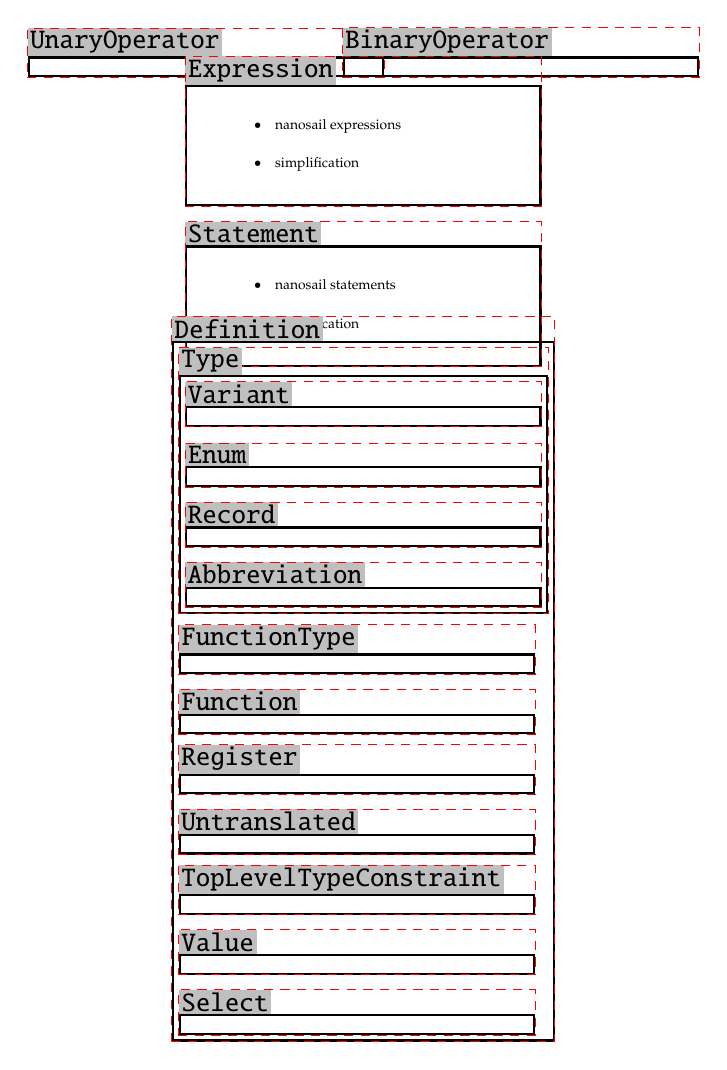
\begin{tikzpicture}[
  module box/.style={thick,draw,minimum width=4.5cm,inner sep=2pt},
    module tag/.style={fill=gray!50,line width=0pt,inner sep=1pt},
    module group/.style={inner sep=0mm,line width=0pt,dashed,red,draw},
  ]

  \module[id=ast-unaryoperator,name=UnaryOperator,at={(-2,0)}]{ }
  \module[id=ast-binaryoperator,name=BinaryOperator,at={(2,0)}]{}

  \module[id=ast-expression,name=Expression,at={(0,-1)}]{
    \begin{itemize}
      \item nanosail expressions
      \item simplification
    \end{itemize}
  }

  \module[id=ast-statement,name=Statement,below=ast-expression]{
    \begin{itemize}
      \item nanosail statements
      \item simplification
    \end{itemize}
  }

  \module[id=ast-definition-variant,name=Variant,below last,submodule of=ast-definition-type]{}
  \module[id=ast-definition-enum,name=Enum,below last,submodule of=ast-definition-type]{}
  \module[id=ast-definition-record,name=Record,below last,submodule of=ast-definition-type]{}
  \module[id=ast-definition-abbreviation,name=Abbreviation,below last,submodule of=ast-definition-type]{}
  \supermodule{id=ast-definition-type,name=Type}
  
  \module[id=ast-definition-functiontype,name=FunctionType,below=ast-definition-type,submodule of=ast-definition]{}
  \module[id=ast-definition-function,name=Function,below last,submodule of=ast-definition]{}
  \module[id=ast-definition-register,name=Register,below last,submodule of=ast-definition]{}
  \module[id=ast-definition-untranslated,name=Untranslated,below last,submodule of=ast-definition]{}
  \module[id=ast-definition-topleveltypeconstraint,name=TopLevelTypeConstraint,below last,submodule of=ast-definition]{}
  \module[id=ast-definition-value,name=Value,below last,submodule of=ast-definition]{}
  \module[id=ast-definition-select,name=Select,below last,submodule of=ast-definition]{}
  \addsubmodule{ast-definition}{ast-definition-type}


  % \node[module group,fit=(ast-expression)(ast-statement)(ast-unaryoperator)(ast-binaryoperator)] { };
  \supermodule{id=ast-definition,name=Definition}
\end{tikzpicture}

\end{document}